
%%%%%%%%%%%%%%%%%%%%%%% file typeinst.tex %%%%%%%%%%%%%%%%%%%%%%%%%
%
% This is the LaTeX source for the instructions to authors using
% the LaTeX document class 'llncs.cls' for contributions to
% the Lecture Notes in Computer Sciences series.
% http://www.springer.com/lncs       Springer Heidelberg 2006/05/04
%
% It may be used as a template for your own input - copy it
% to a new file with a new name and use it as the basis
% for your article.
%
% NB: the document class 'llncs' has its own and detailed documentation, see
% ftp://ftp.springer.de/data/pubftp/pub/tex/latex/llncs/latex2e/llncsdoc.pdf
%
%%%%%%%%%%%%%%%%%%%%%%%%%%%%%%%%%%%%%%%%%%%%%%%%%%%%%%%%%%%%%%%%%%%


\documentclass[runningheads,a4paper]{llncs}

\usepackage{amssymb}
\setcounter{tocdepth}{3}
\usepackage{booktabs}
\usepackage{graphicx}
\usepackage{epstopdf}
\usepackage[utf8]{inputenc}
\usepackage[T1]{fontenc}
\usepackage{lmodern}

\usepackage{url}
\urldef{\mailsa}\path|loic.tetrel@mail.mcgill.ca|    
\newcommand{\keywords}[1]{\par\addvspace\baselineskip
\noindent\keywordname\enspace\ignorespaces#1}

\begin{document}

\mainmatter  % start of an individual contribution

% first the title is needed
\title{Assignment 1 : Performance of Gaussian Mixture Models (GMMs) with Expectation-Maximization (EM) algorithm}

% a short form should be given in case it is too long for the running head
\titlerunning{Gaussian Mixture Models (GMMs) with Expectation-Maximization (EM) algorithm}

% the name(s) of the author(s) follow(s) next
%
% NB: Chinese authors should write their first names(s) in front of
% their surnames. This ensures that the names appear correctly in
% the running heads and the author index.
%
\author{Loïc Tetrel}
%loic.tetrel@mail.mcgill.ca
\authorrunning{Gaussian Mixture Models with Expectation-Maximization algorithm}
% (feature abused for this document to repeat the title also on left hand pages)

% the affiliations are given next; don't give your e-mail address
% unless you accept that it will be published
\institute{McGill University\\
845 Rue Sherbrooke O, QC H3A 0G4, Montréal, Canada\\
%The purpose of this paper is to summarize the main contributions in the area of sensorless registration for 3D echography. Because the registration is performed using the echographic noise called speckle, the problematic is really complex due to the nature of speckle in ultrasound. We will see that the registration of echographic images has to be performed by dividing the main problem in the estimation of out-of-plane ($z, \theta_x, \theta_y$) and in-plane ($x, y, \theta_z$) parameters. This will lead to many discussion like the influence on the rotation of the probe, the question of real tissue imagery and the reconstruction of the frame's  pose.
%\keywords{3D ultrasound. Statistics of speckle. RF signal. Sensorless rigid registration.}
%\end{abstract}
\mailsa\\
}

%\toctitle{Sensorless registration of echographic images for 3D ultrasound}
\maketitle

%\begin{abstract}

\section{Introduction}

In the area of computer vision Bayes theorem has been widely used, indeed the use of a prior help us to solve the solution. So what is the probability of an hypothesis $\mathcal{H}$ given our data $D$ ?
\begin{equation}
p(\mathcal{H}|D)=\frac{p(D|\mathcal{H})\times p(\mathcal{H})}{p(D)}
\end{equation}
Most of the time, we need to model the Likelihood function $p(D|\mathcal{H})$. This is the goal of this assignment and we will try to answer the following question : given a set of obervations, how do we model a probability density ?\par
We will frst study the case of Gaussian Mixture Model (GMM) in sec. \ref{sec:gmm}, then we will see how can we select the best number of gaussian for GMM if we don't know its in sec. \ref{sec:modelselection}, finally we will conclude with the evaluation of the GMM approach compare to a simple K-mean algorithm.

\section{GMM with EM algorithm}\label{sec:gmm}
\subsection{Theory}
There are two ways to estimate a probability density function (pdf) : parametric estimation and non-parametric estmation. We will focus on parametric estimation, so a finite number of parameters for the pdf.
Gaussian model is realy usefull and is a good approximation for many true density, however many practical cases involve multi-modal densities (see fig. \ref{fig:gmm}). 

\begin{figure}
\centering
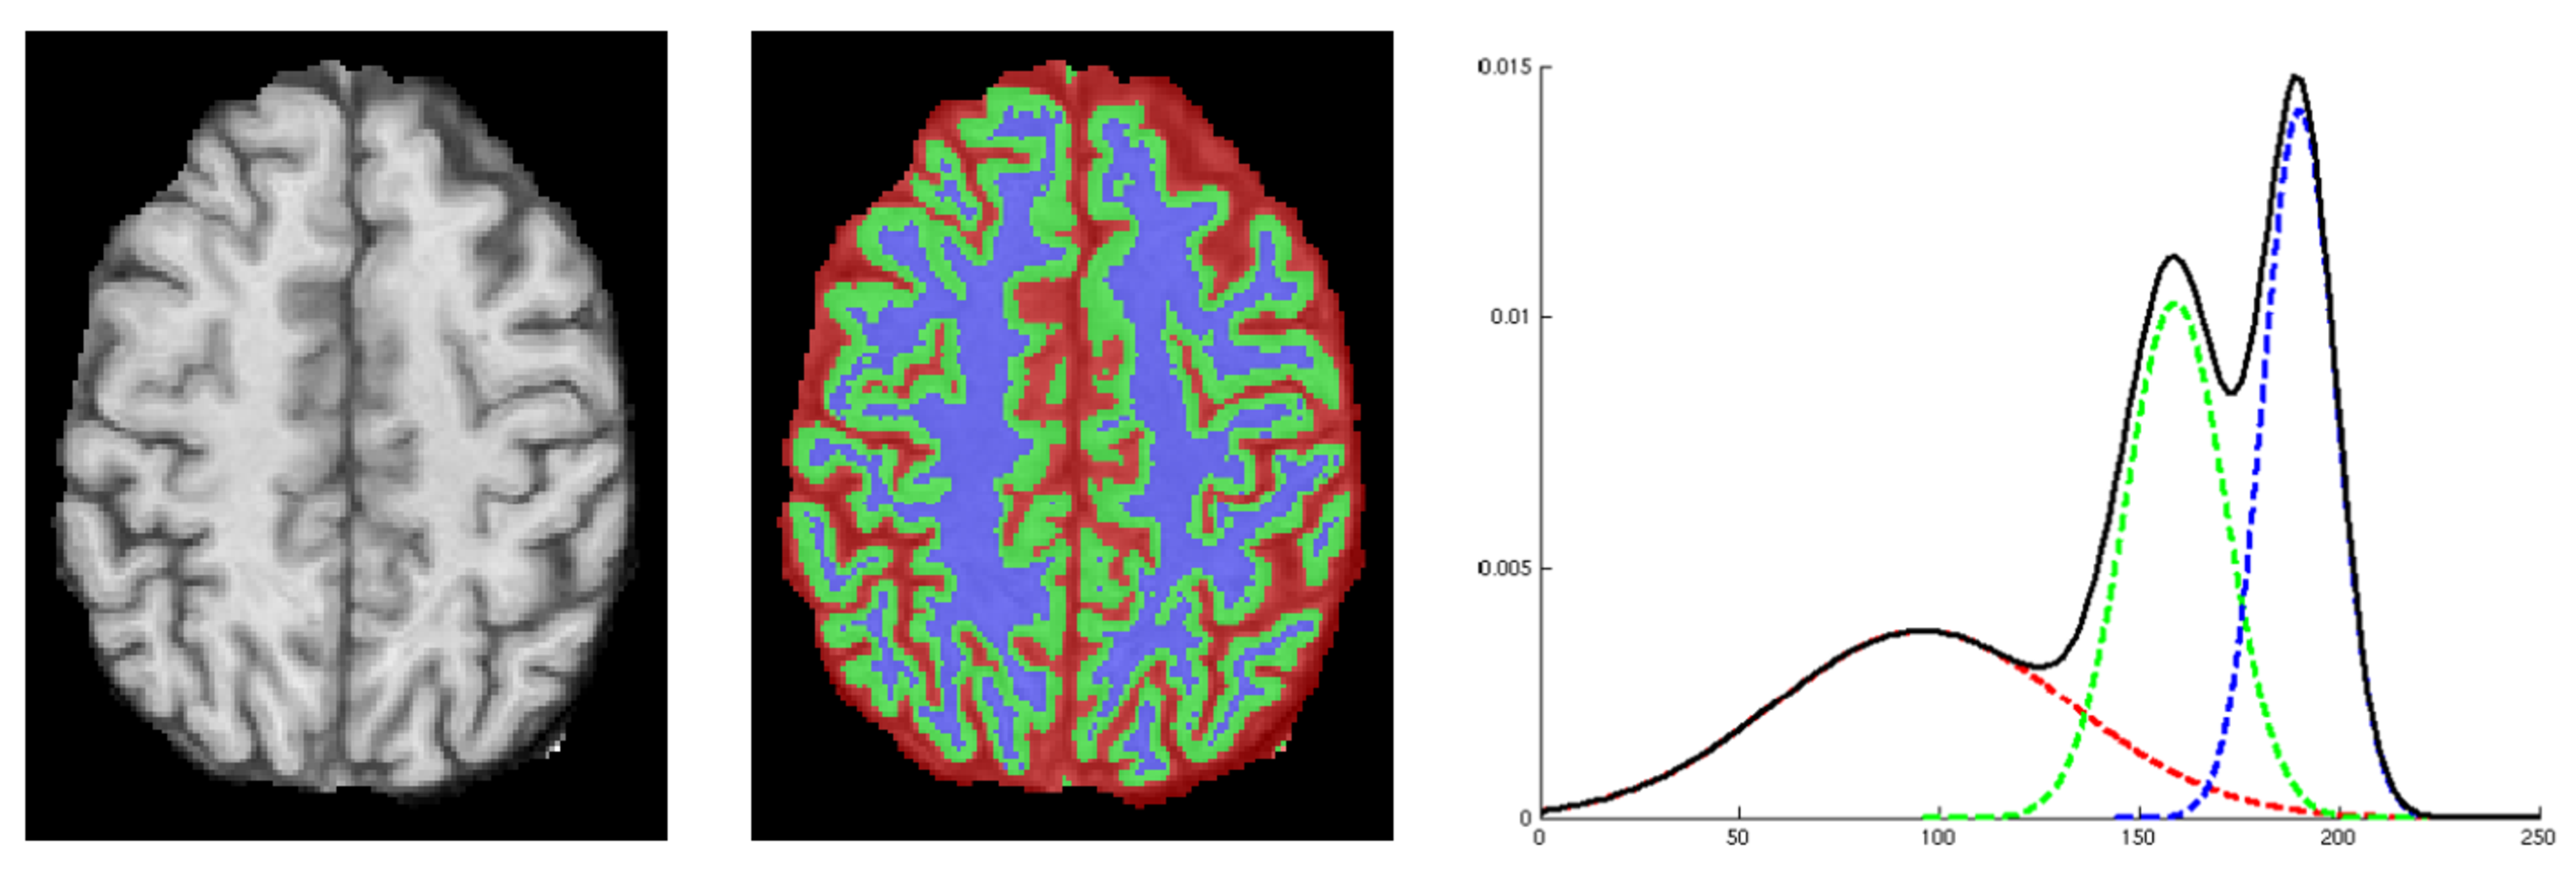
\includegraphics[height=4cm]{Figures/gmm}
\caption{Example of the use of GMM for image brain segemntation. Extracted from \cite{Arbel16}.}
\label{fig:gmm}
\end{figure}

GMM is well suited to extract a multi-modal density and has been used in many clustering task. Indeed, it allows us to represent densities as
weighted sum (or mixture) of $K$ multiple Gaussians. We assign a gaussian $\mathcal{N}(\mu_k,\sigma_k)$ to each cluster $k$ with the position of the center $\mu_k$ and width $\sigma_k$, finally we weight this gaussian by a factor $\alpha_k$ :
\begin{equation}
f(x|\Theta)=\sum^K_{k=1}\alpha_k\times\mathcal{N}(x;\mu_k,\sigma_k)
~~\textrm{with}~~
\Theta = \{\alpha_1,...,\alpha_k,\mu_1,...,\mu_k,\sigma_1,...,\sigma_k \}
\label{eq:gmm}
\end{equation}\par

\textbf{First assumption.} The first assumption that we make is the number $K$ of gaussian, so given $K$ what is the best parameter $\Theta$ that we can extract from the image ? 
Using eq. \ref{eq:gmm} and if our samples $\mathcal{X}=\{x_1,...,x_N\}$ are i.i.d we can try to maximize the likelihood which gives us :

\begin{equation}
\Theta^*= \arg\max_{\Theta} \sum^N_{i=1}\log \big(\sum^K_{k=1}\alpha_k\times\mathcal{N}(x;\mu_k,\sigma_k)\big)
\label{eq:likelihoodgmm}
\end{equation}

The eq. \ref{eq:likelihoodgmm} is complicated because it contains a $\log$ of summation, so the idea is to introduce a hidden parameter $\mathcal{Y}=\{y_1,...,y_N\}$ the label of our samples.
The introducing of $\mathcal{Y}$ will provide the likelihood of class $k$ (parametrized by the $k^{th} $gaussian) at each sample, this is the basis of what we call the EM algorithm. 
It is an iterative procedure :
\begin{enumerate}
\item We estimate $y_i$ based on current estimate of parameters (E-step)
\item We find the parameters $\Theta$ that maximizes expectation of log-likelihood (M-step)
\end{enumerate} 
This process is repeated until convergence because we are guaranteed to converge at least a local maximum.\par
\textbf{Second assumption.} The second assumption made is the label $y_i$ for each sample, a common use is to label with a uniform density based on the number of class $K$. The initialization of $y_i$ will start the EM algorithm (after M-step, E-step, M-step,... until convergence).\par
\textbf{Third assumption.} The last assumption is the convergence criteria. It is important because we don't want to lose information if we stop to early and we don't want to overfit the data if it stop to late.

\subsection{Evaluation of the EM/GM}
The experiments where performed on a MSI laptop with a processor Intel i5 - 2.3GHz and Matlab 2012.a.
The EM/GMM was designed with matrixes and vectorizations to speed up the computation time. There are two possible ways to initialiaze the labels : randomly (what I used during all the parts) or assigning labels using quantiles of features. The sum of log-likelihoood was computed using the GMM formula (eq. \ref{eq:gmm}). 
As a criteria of convergence, I choosed to stop when $\sum\log_{lklh}(i) - \sum\log_{lklh} (i-1) < 0.01$. The labelisation was performed using the maximum log of :
\begin{equation}
\alpha_{y_i}^t\times\mathcal{N}(x_i;\nu_{y_i}^t,\sigma_{y_i}^t)
\end{equation}

Using the GMM for $2, 4$ and $6$ gaussians for all the features (grey, ab of Lab and rgb) gives the results summarized in fig. 2.
\begin{figure}
\centering
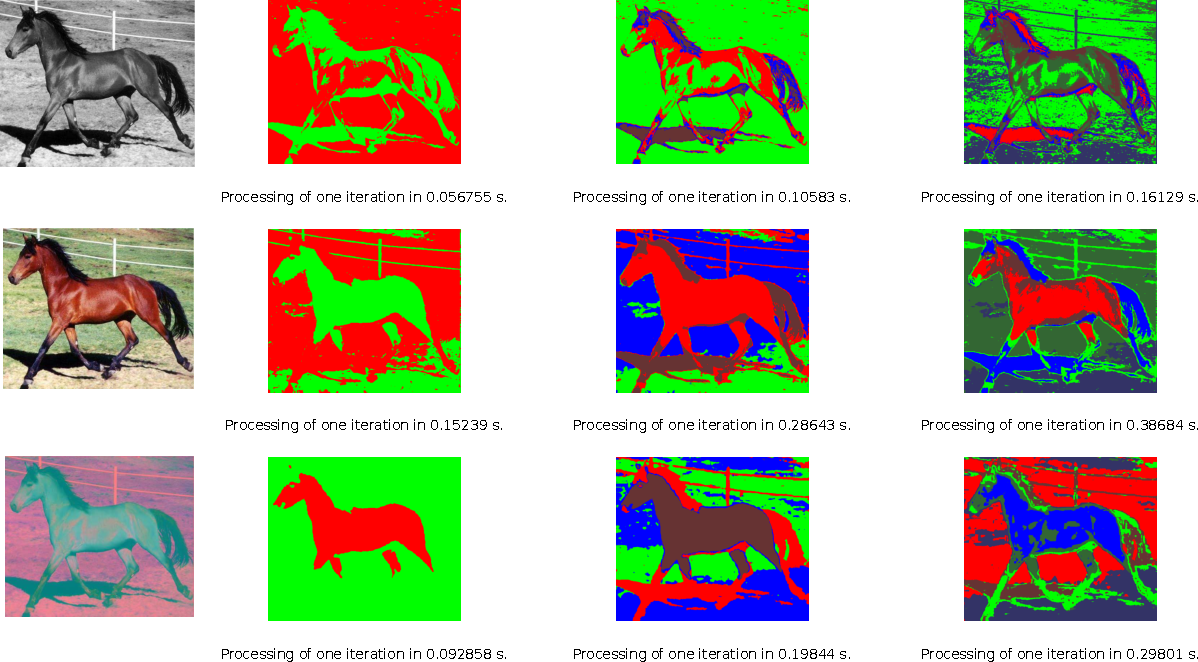
\includegraphics[height=7cm]{Figures/labels_horse}
\caption{Segementation of the image `horse' for (up to down) grey-space, rgb and lab with (left to right) $2,4$ and $6$ gaussians.}
\end{figure}
\par Obviously, the more they are gaussians, the more the image is divided. It is interesting to see that from 4 gaussians we can detect the barrier and after 6 gaussiand we are sure to detect the ground (and the difference between grass and earth). I think that the best feature space is rgb, because it's a good mix between the smoothness of Lab and the noise of grey-space. The horse is really prone to noise for the grey space, and it failed when we want to detect all the horse. But, it's good to have a high resolution of segmentation (this can be seen with the mane's horse). In the other hand, the Lab space tends to create smooth clusters inside the image. Of course, rgb space takes more time to compute because we have 3 caracteristics and it takes three times more time to compute one EM iteration. One drawback of the GMM is that we don't know what the label is. For example in the horse image the horse isn't not always at the same color.

\par We can look more closely to the shape of the different gaussians. For the grey space, I also computed the pdf of each label using a parzen window (with a gaussian kernel) bolded in the left figure. This represent the posteriori probability of the label $p(k|x)$ and it is interesting to see that the result is not gaussian because this probability takes into account the frequency of the pixels in the image.

\begin{figure}
\centering
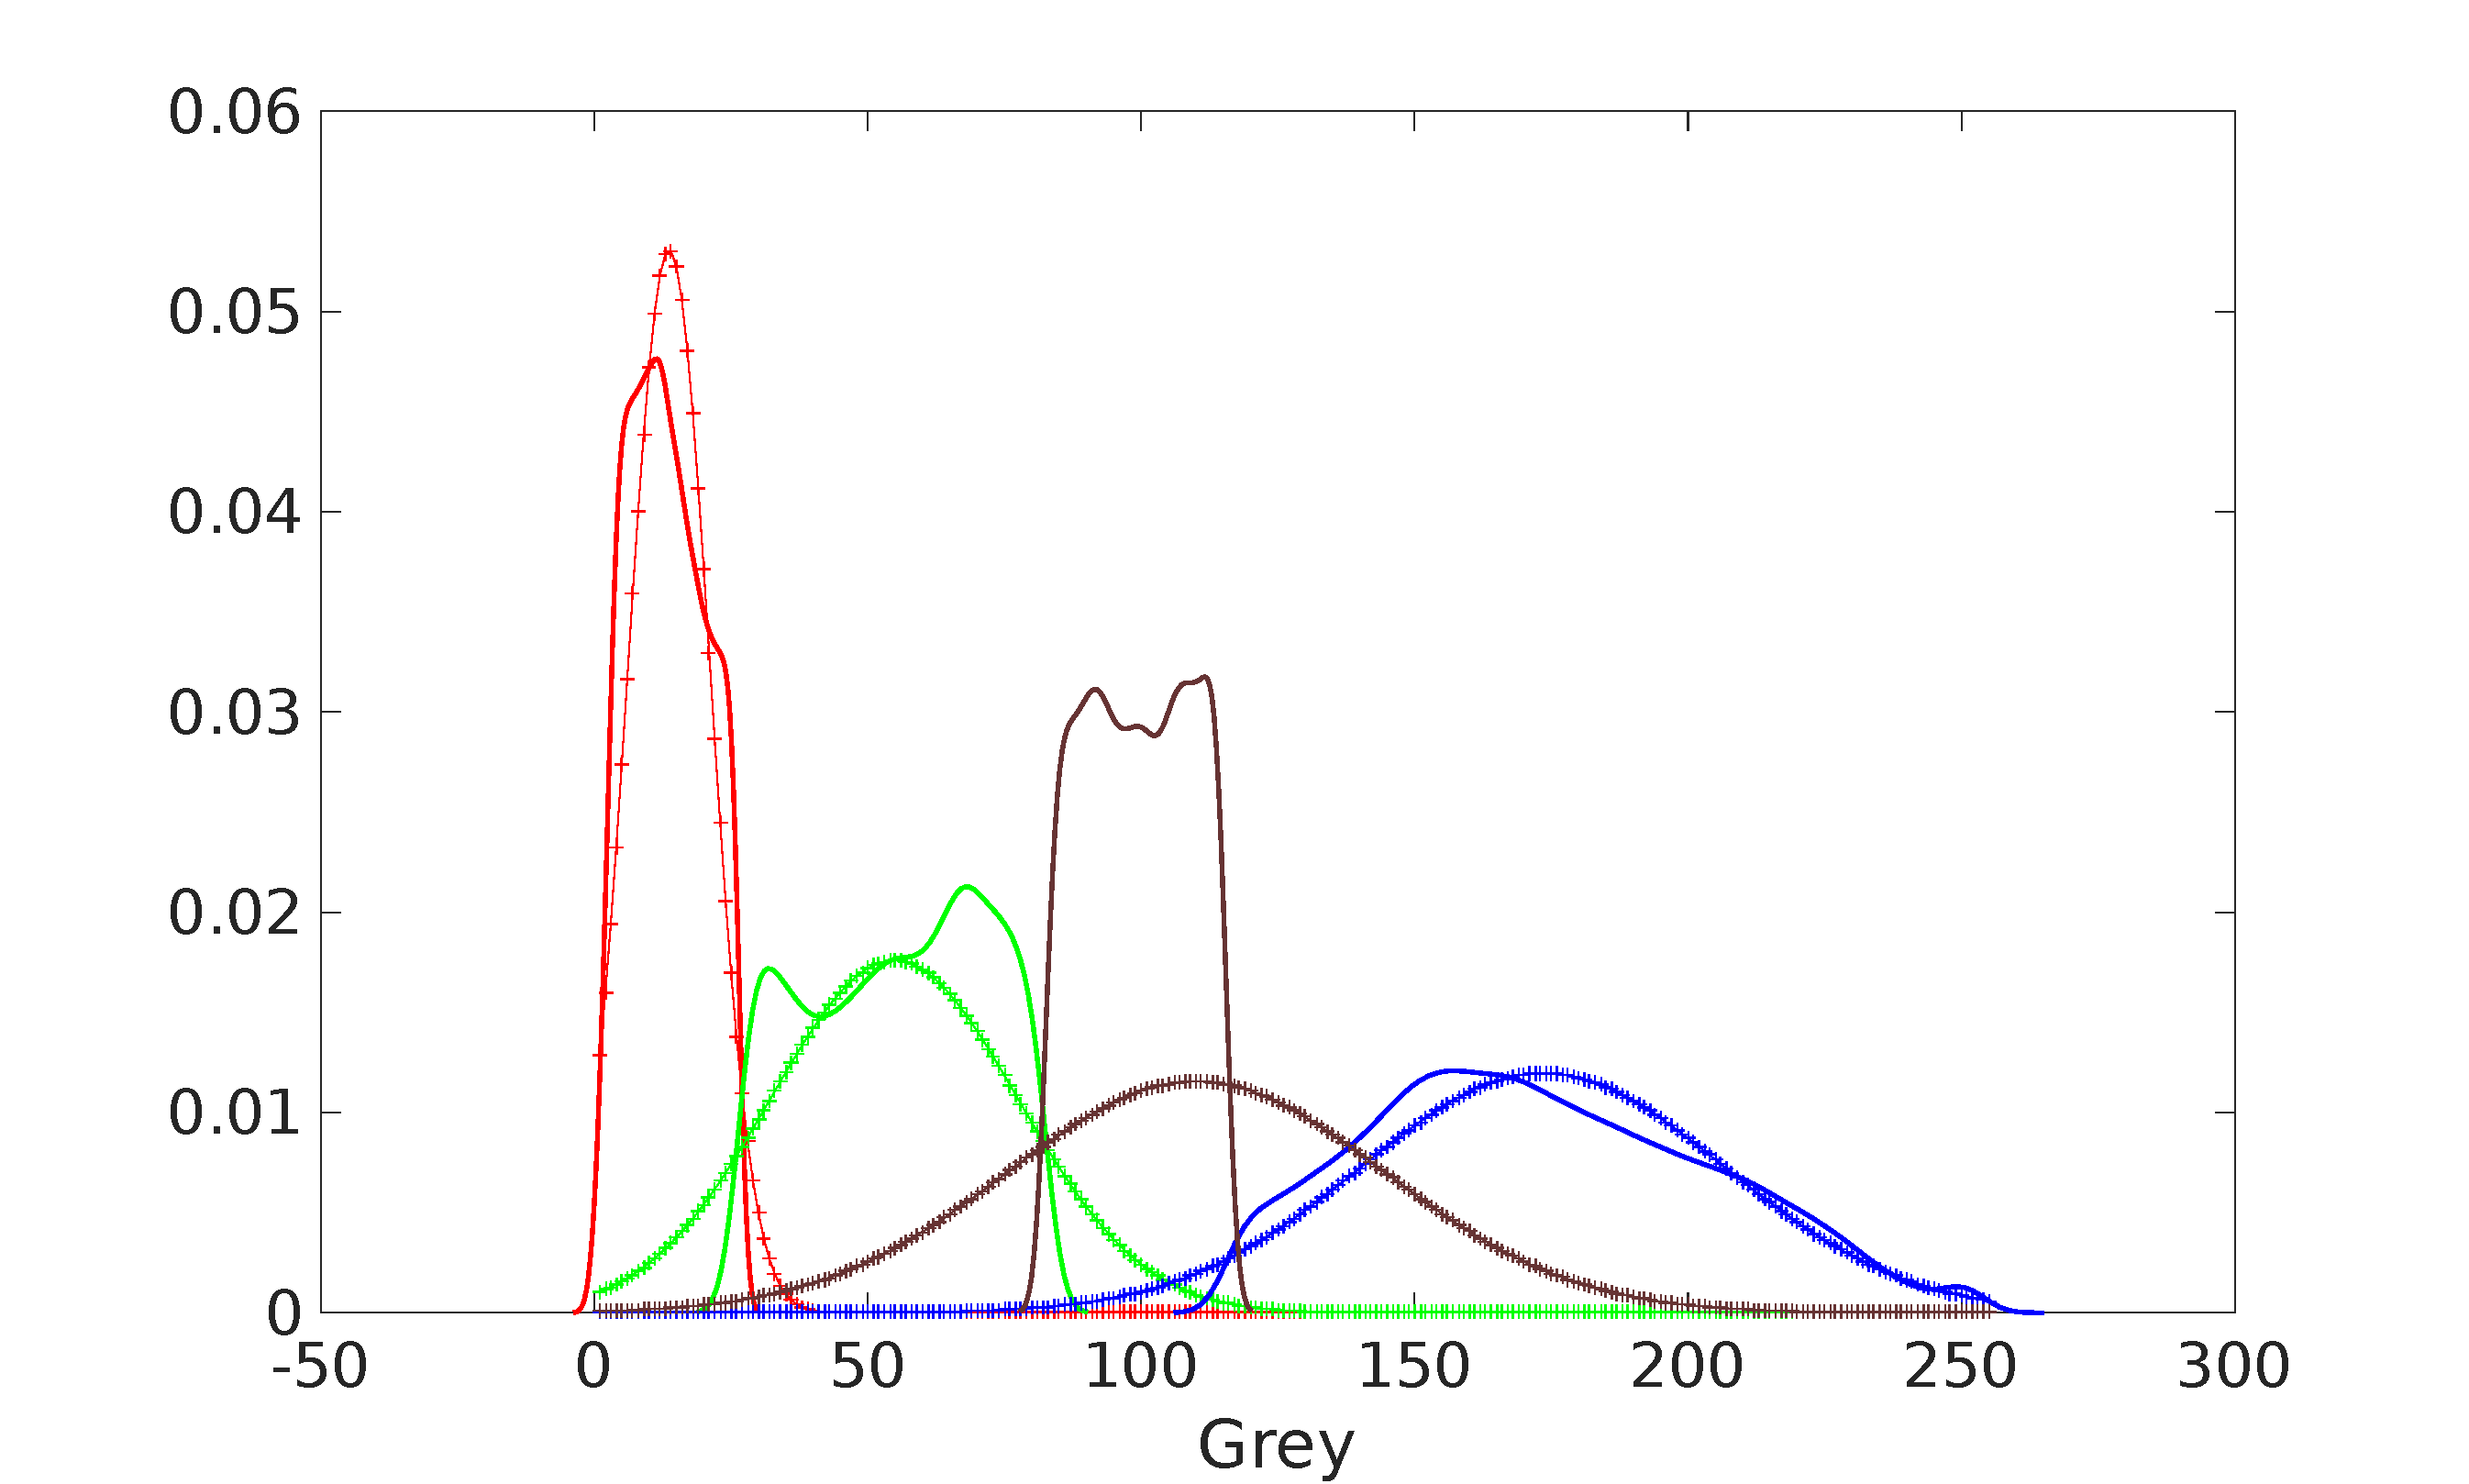
\includegraphics[height=3cm]{Figures/plot_1carac}
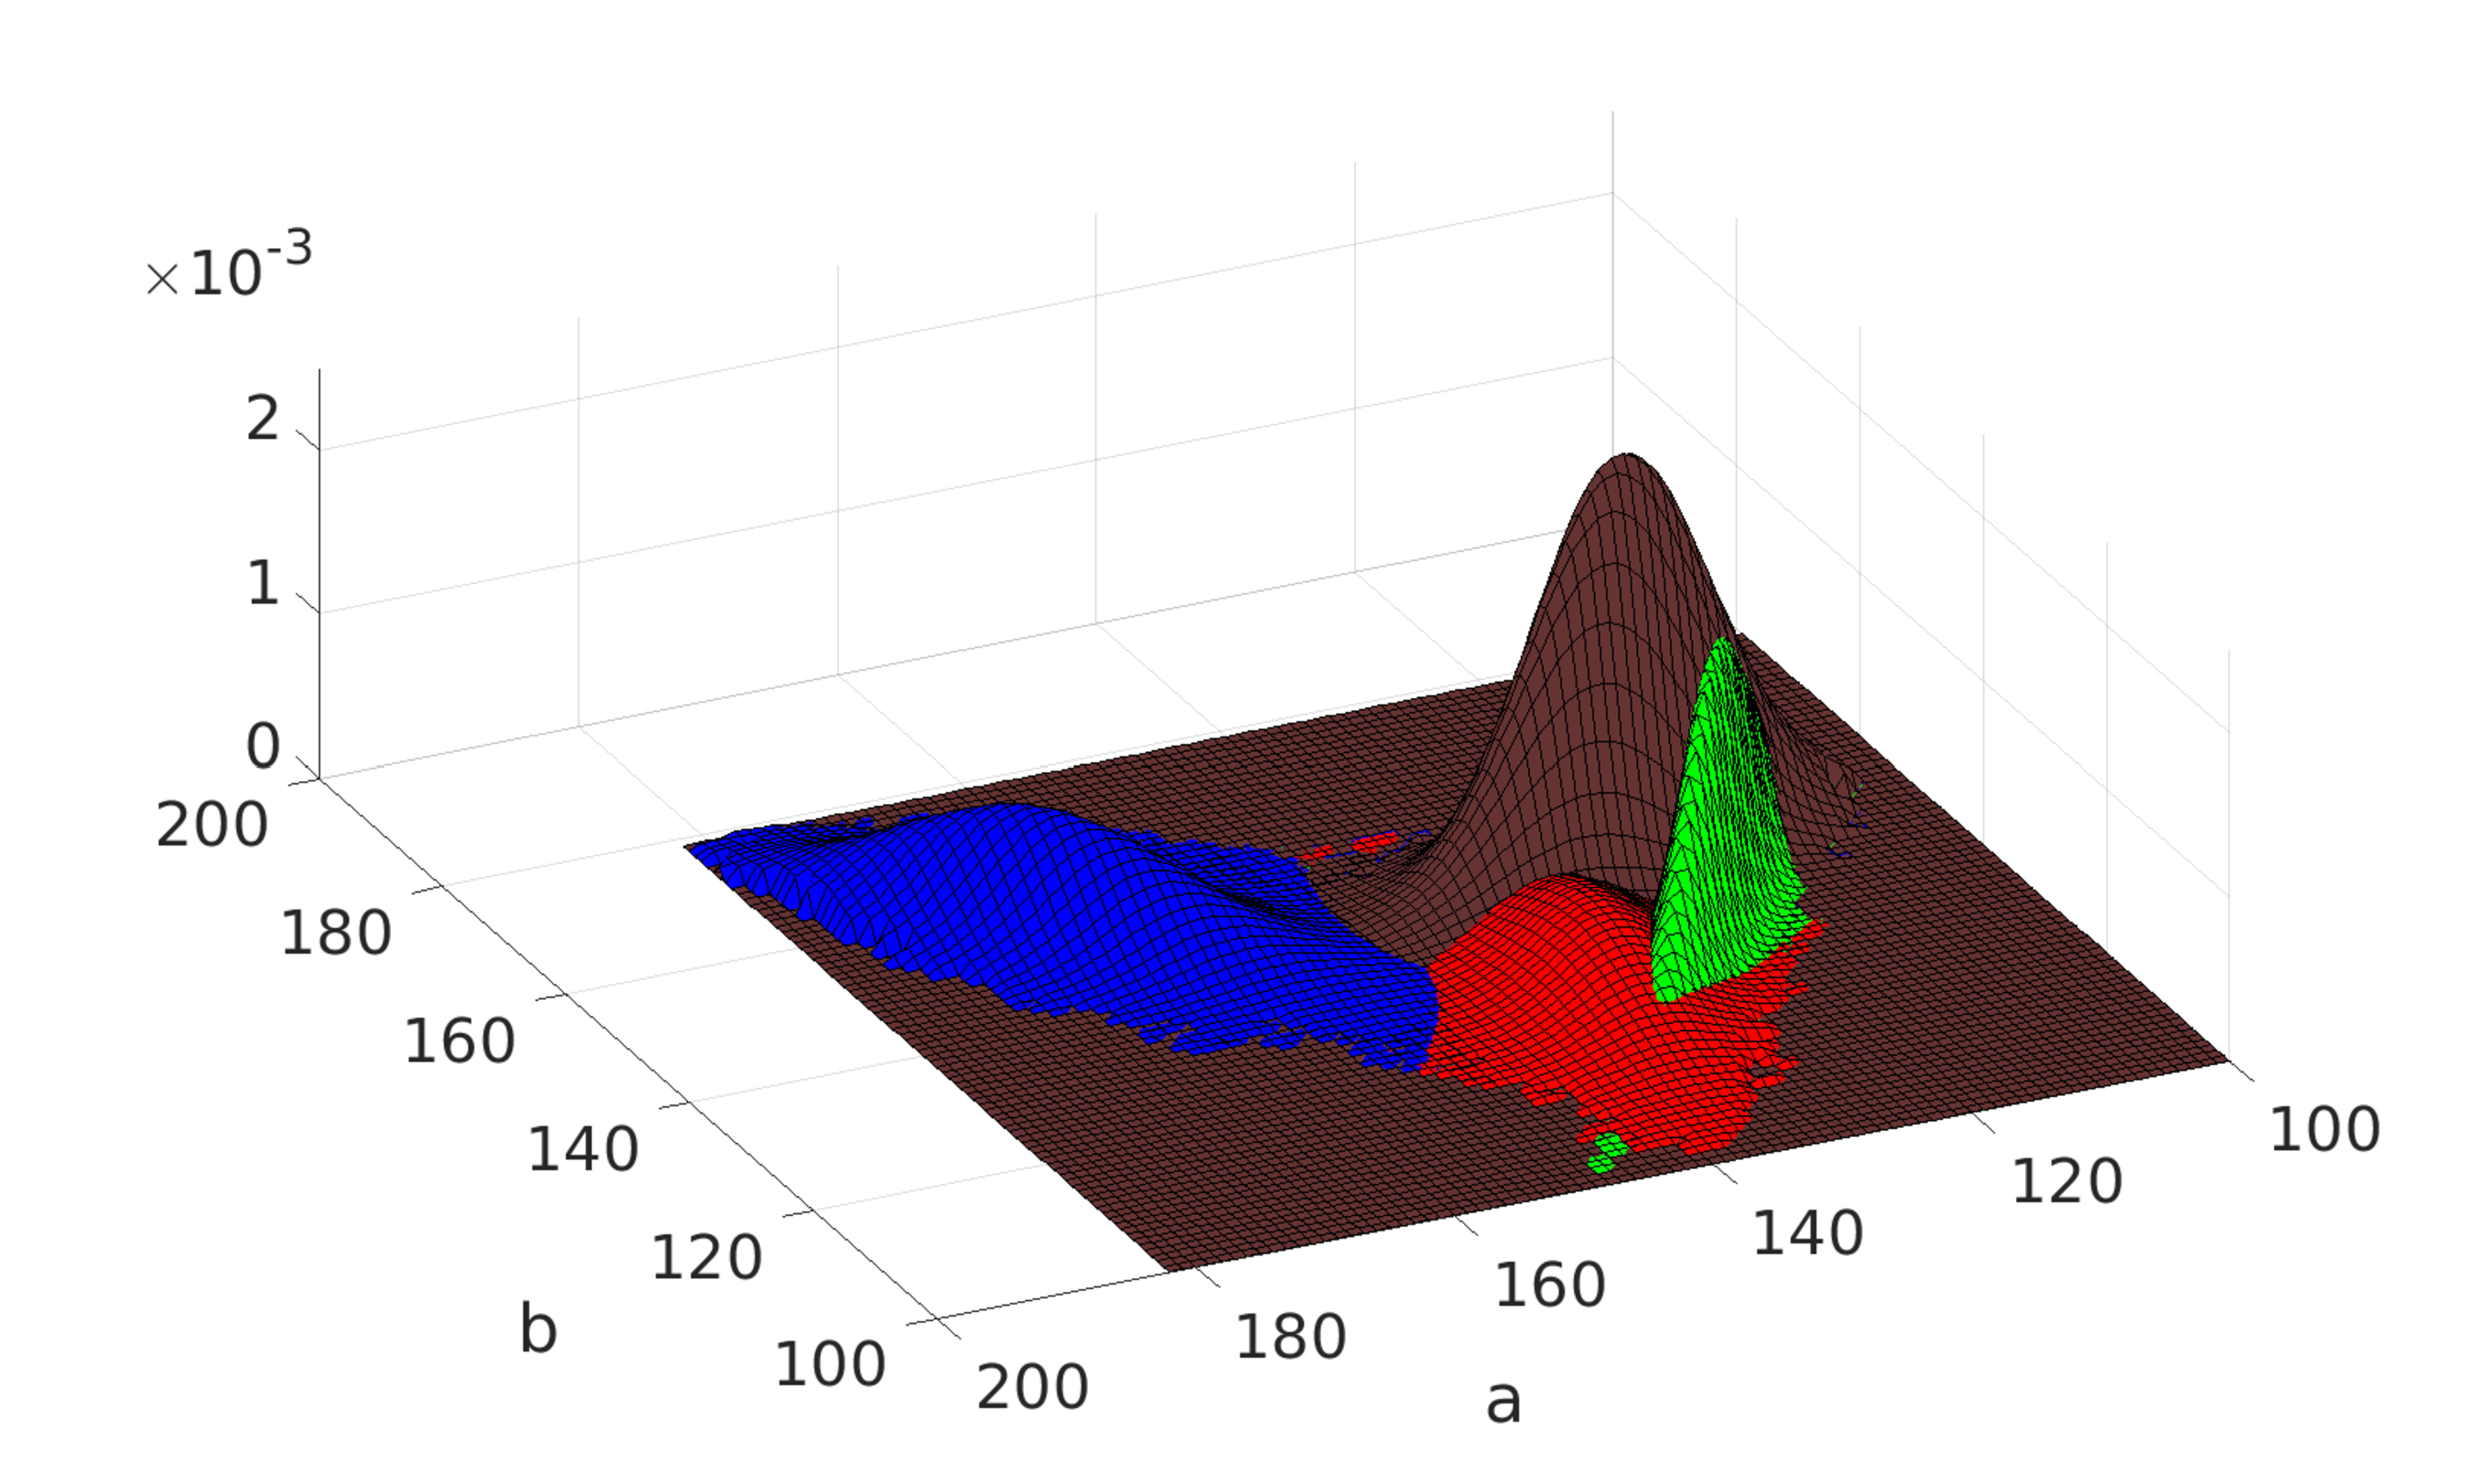
\includegraphics[height=3cm]{Figures/plot_2carac}
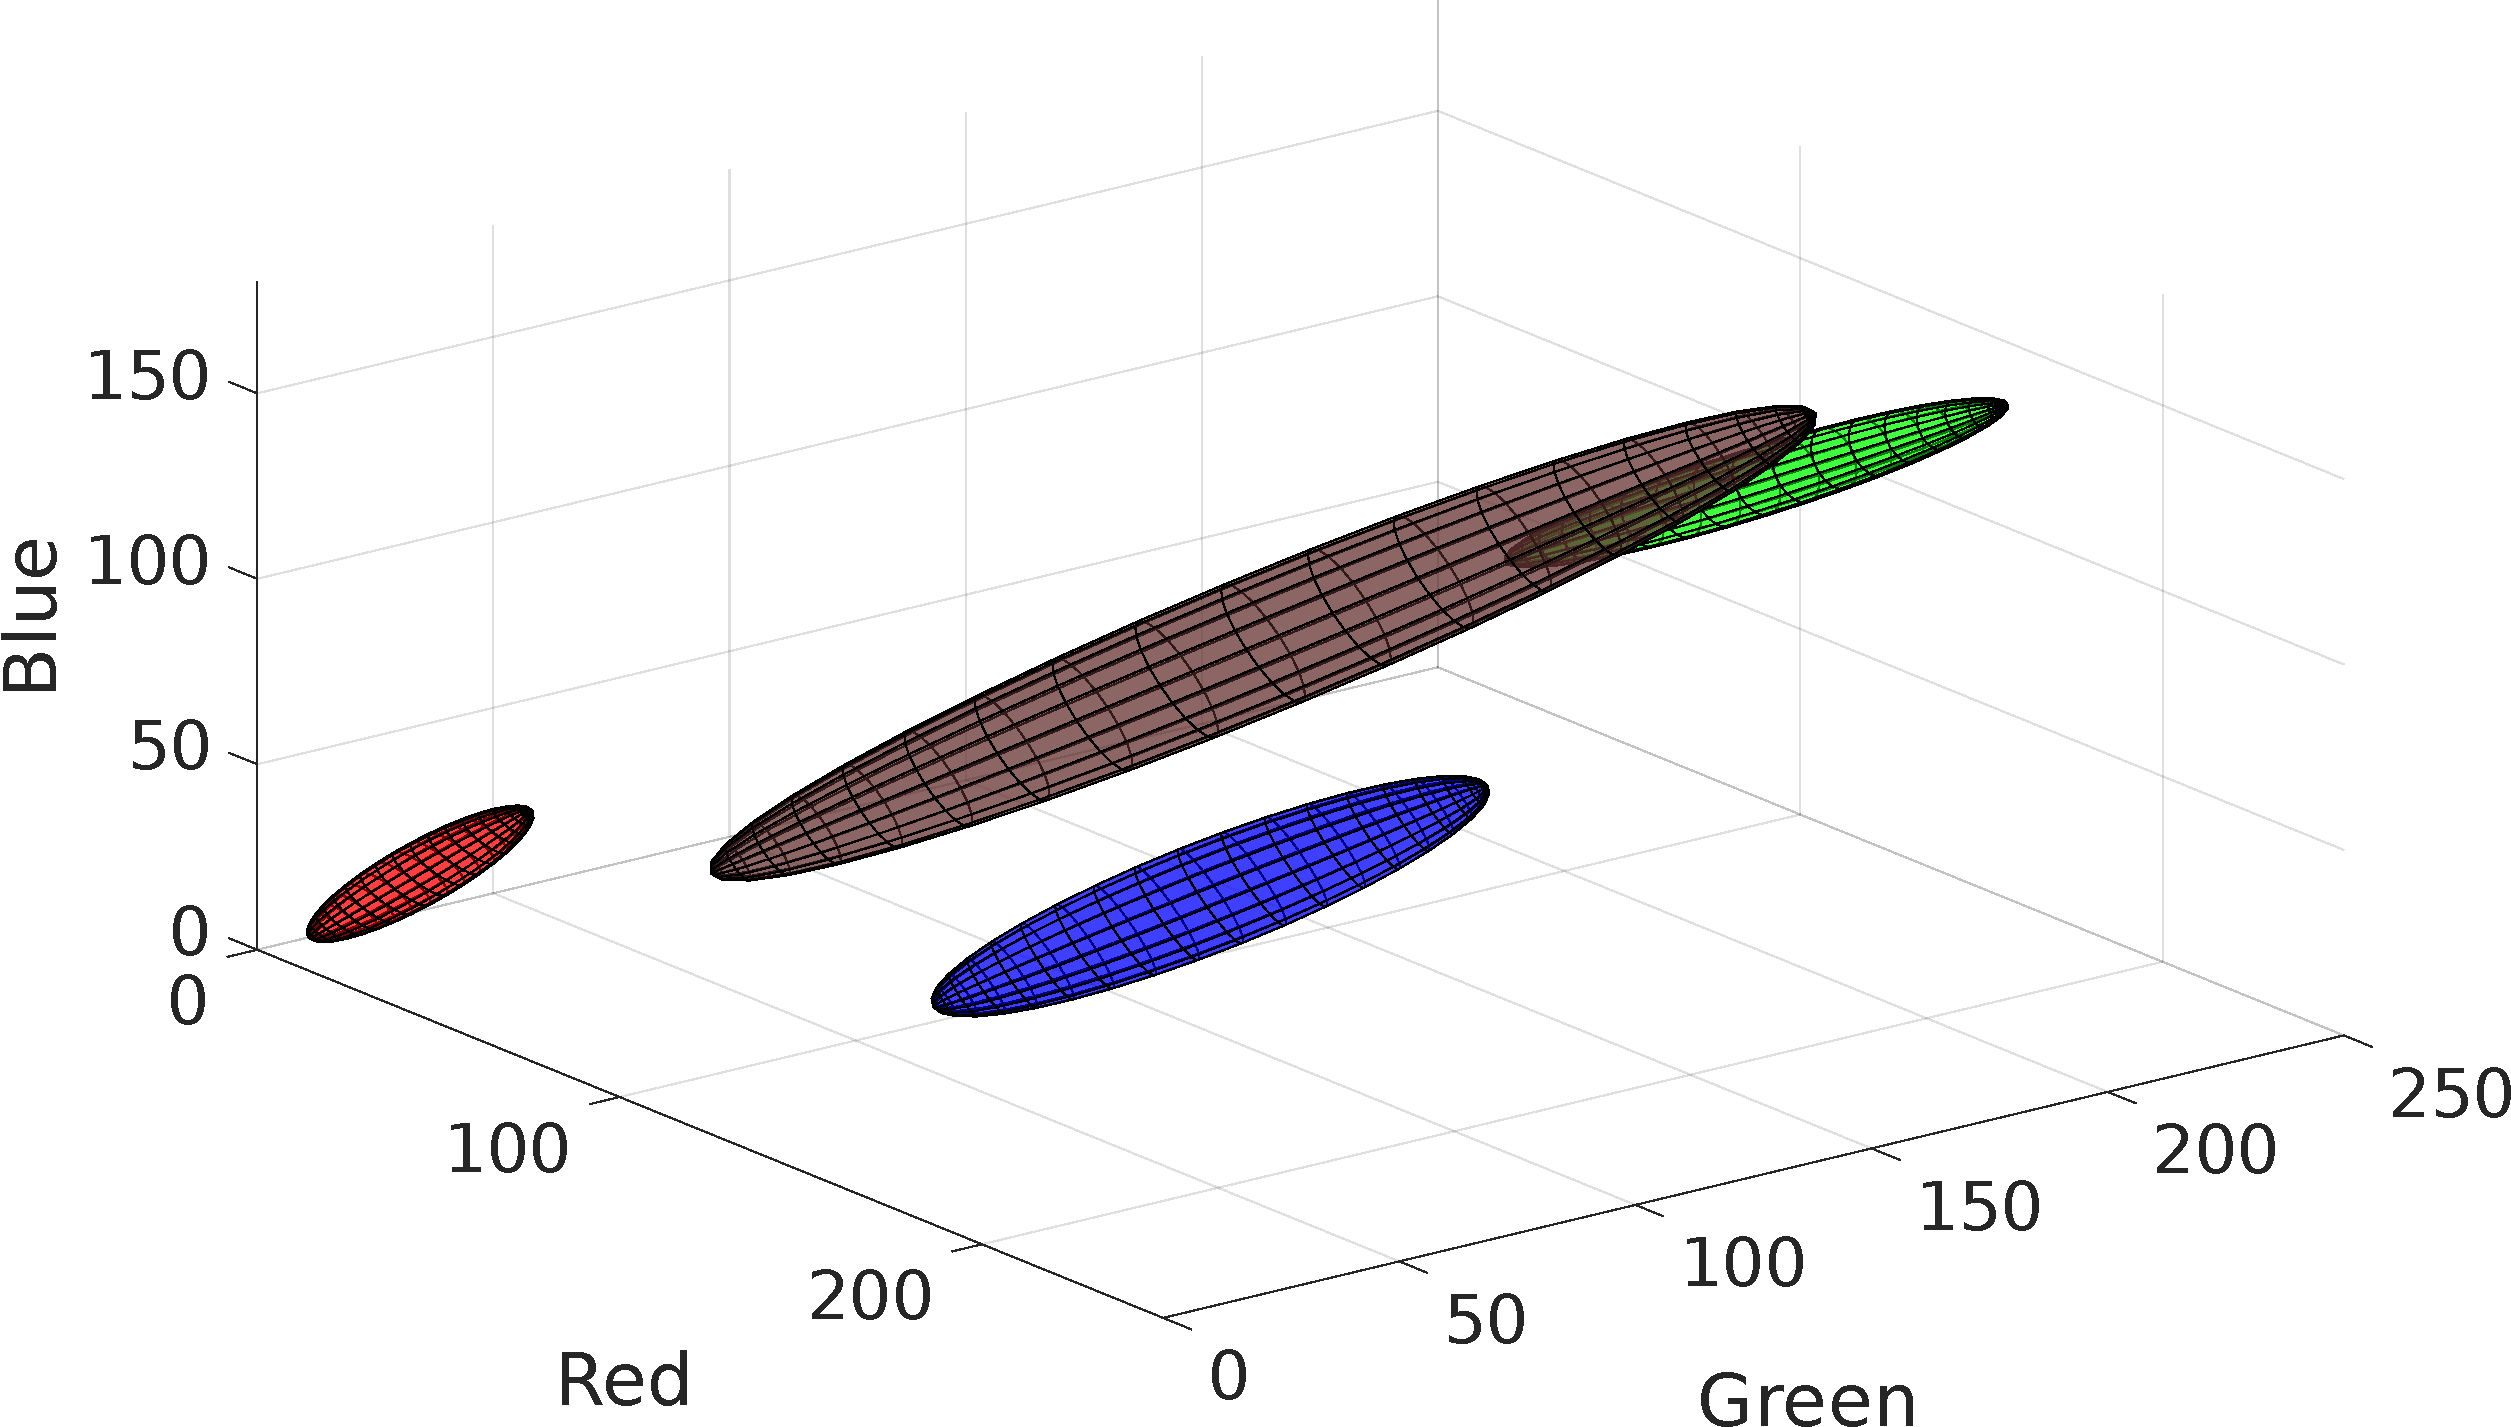
\includegraphics[height=3cm]{Figures/plot_3carac}
\caption{Plot of the gaussians for grey space (left), Lab space (right) and rgb space (bottom).}
\end{figure}

\par Finaly, it's interesting to look at the evolution of the max log-likelihood of the GMM. The choice of the criteria of convergence is important because if it is badly chosen we risk to convergence on the ``bumps''. Moreover, this figure shows that we assure to converge at a maximum.

\begin{figure}
\centering
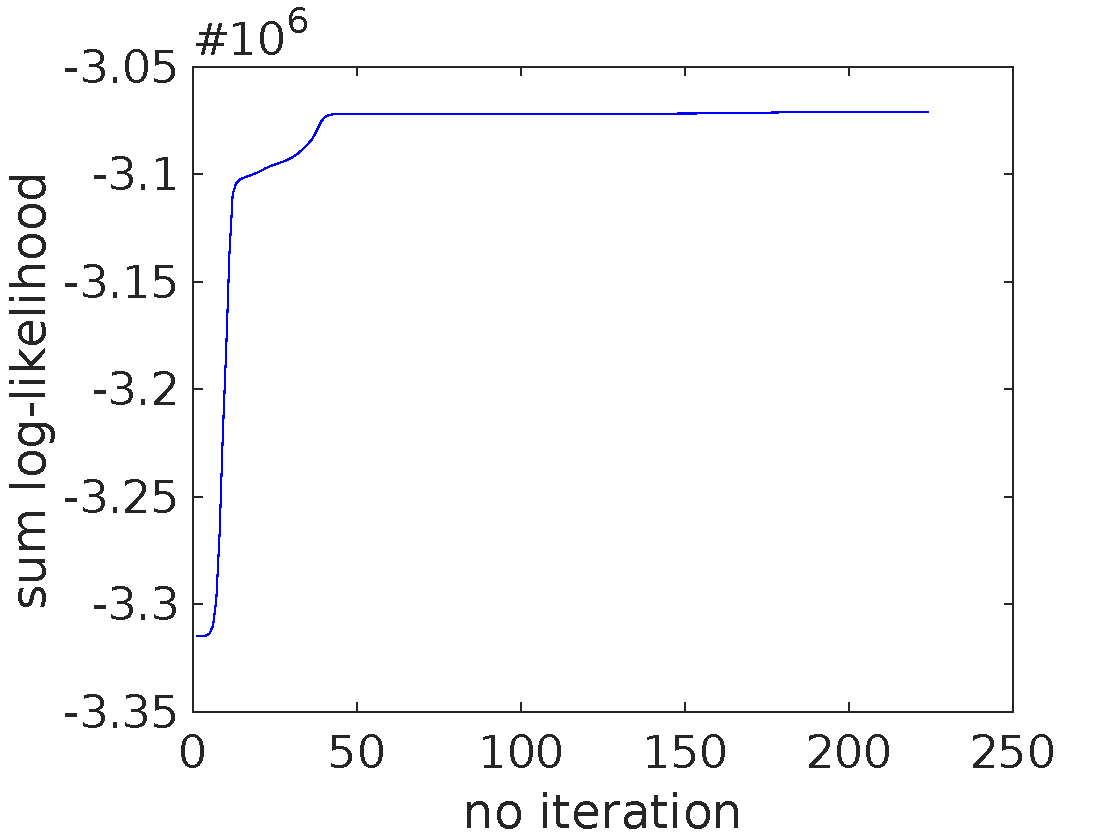
\includegraphics[height=4cm]{Figures/likelihood}
\caption{Convergence of the sum of log-likelihood.}
\end{figure}
 
\section{Model selection}\label{sec:modelselection}
Because in the ``real'' world we don't know how many gaussians we need to choose, it is common to perform a training and testing on the model. To test our model, we can use methods like cross validation or BIC criteria.
\subsection{Cross validation}
In the spirit of machine learning, a $k$-fold cross validation consist of dividing our data into $k$ boxes. In this assignment $k-1$ boxes will be used to train our model and the last $k$th box will be used to test the model. To say if the model is good or not, I will calculate $mean(\log(likelihood_{GMM}))$. 
\begin{figure}
\centering
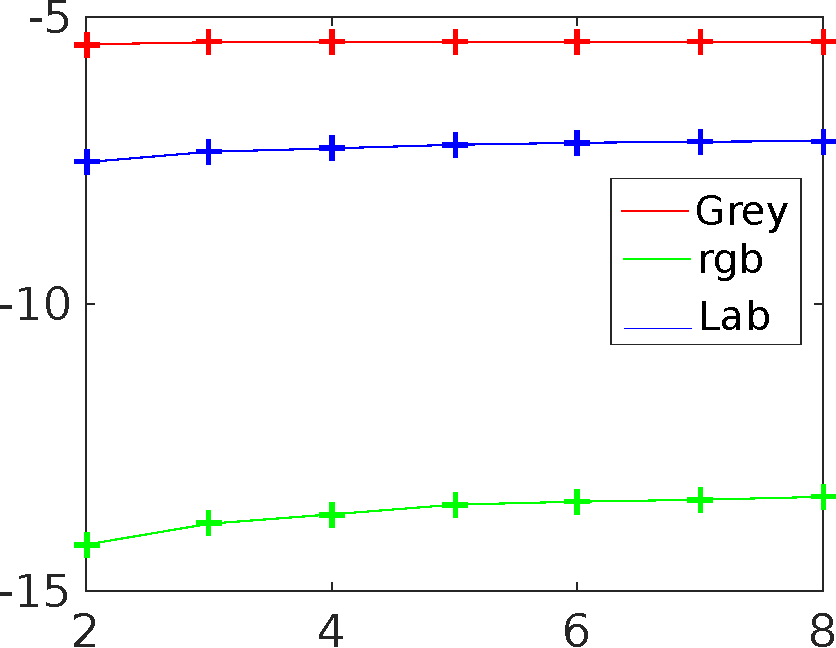
\includegraphics[height=3cm]{Figures/mean_lklh}
\caption{Evolution of the mean likelihood with the number of gaussians.}
\end{figure}
\par It's also interesting to see the influence on all the likelihood data and not just the mean, because even if the mean is really powerful it tends to generalize to much the data. I calculated the mean log-likelihood score at each pixel, the mean was performed on the $k-1$ values of the log-likelihood's pixel . The figure shows the mean log-likelihood score at each pixel for the worth component (2 gaussians) and the best component (8 gaussians), we it can be seen that the overall likelihood is better for the highest number of gaussians.
\begin{figure}
\centering
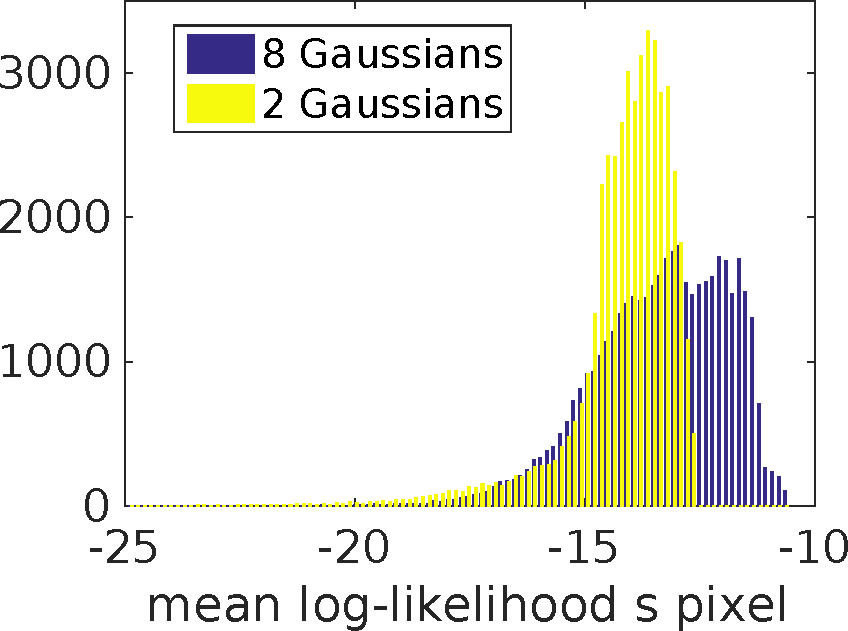
\includegraphics[height=3cm]{Figures/hist_lklh}
\caption{Histograms of the mean likelihood for all pixels}
\end{figure}

\subsection{Bayesian information criterion}

Bayesian information criterion (BIC) \cite{wit2012all} is in the spirit of occum razor because it penalizes complex model, it can be formulated as follow :
\begin{equation}
BIC \approx -2\sum\ln p(x|\hat{\theta}) + k\ln(n)
\end{equation}
Where $n$ denotes the length of our database and $k$ is the number of parameters of our model.
\par Looking at the figure, we see that contrary to previously, BIC is higher for low number of components. It's understandable because it penalize the high number of gaussians.
Then, I think that the best number of gaussian is the mix between the two previous examples. To have an acceptable likelihood without a complex model, we can choose $5$ or $6$ gaussians. In the case of the horse, I think $6$ is better because it allows to distinguish more the background (grass, earth, barrier...), and the horse (mane, skin, shoe). An idea could be a multi-scale segmentation with first $2$ gaussians to distinguish clearly the horse, and after a second GMM with $6$ gaussians on the two segmented images.

\begin{figure}
\centering
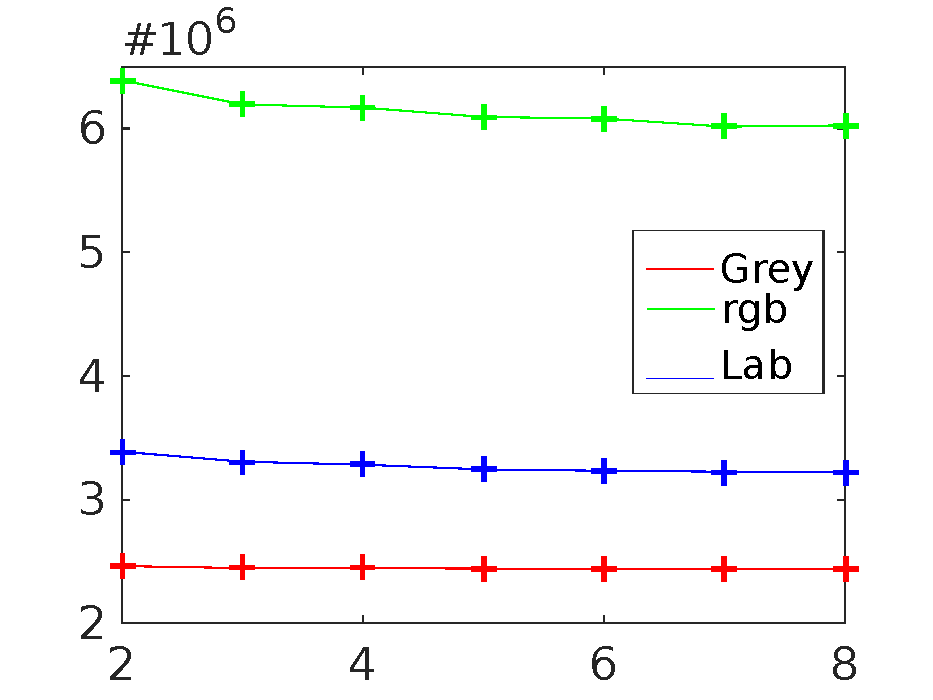
\includegraphics[height=4cm]{Figures/bic}
\caption{Histograms of the mean likelihood for all pixels}
\end{figure}

\section{Conclusion : Segmentation Evaluation}

Using the Weizmann binary segmentation database of 100 images \cite{AlpertGBB07}, we will compare a K-mean segmentation with our GMM for all the feature spaces.
To evaluate a segmentation, commons measure are :
\begin{itemize}
\item Precision which give an overall quality of the segmentation.
\item Recall is the performance for segmenting a ``true'' positive pixel.
\end{itemize}
The F-score combine the previous two measures and can be the harmonic mean of precision and recall :
\begin{equation}
F_1 = 2\times\frac{\textrm{precision}.\textrm{recall}}{\textrm{precision}+\textrm{recall}}
\end{equation}

For this part, we initialize the labels with the quantiles as stated in the part 2.
To see if my GMM is good, I calculated the F-score between their segmentations results and mine. It can be seen that my results follows their results which is a good news !

\begin{figure}
\centering
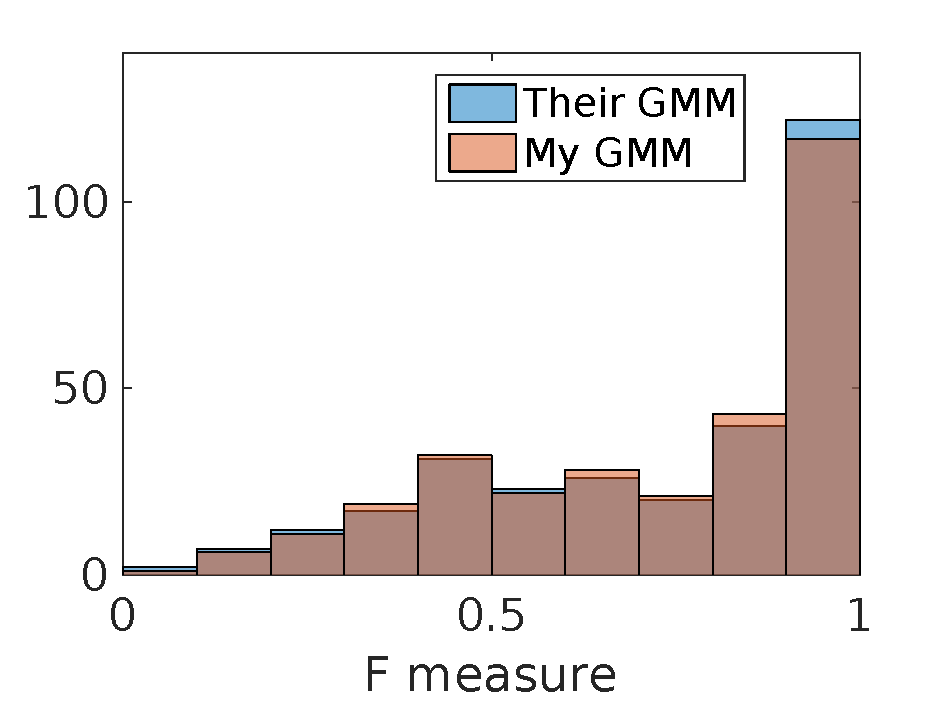
\includegraphics[height=3cm]{Figures/hist_mygmm_their}
\caption{Histograms to compare if my GMM is good}
\end{figure}

\par We have 6 methods that we want to analyse : K-means and EM/GMM, each with three features (grey value, L*a*b and RGB). We will start by a quantitative analysis of the results and we will see som example of images for quantitative analysis.
A Kolmogorov-Smirnof test was performed on all the methods for the three measures of errors. This allowed us to say that the F-measure and the recall has a gaussian distributed law with a confidence level ($p>0.05$), but not the percentage ($p<<0.001$). The gaussian assumption allowed us to perform a 1-way ANOVA (because we have just one group of images) to compare the influence of all the methods.  The recall gives substantially similar measures than the F-measure so we will just focus on the F-measure. 
\par The ANOVA returns that the GMM is significantly better than the K-means ($p<0.05$). In terms of space, Lab isn't significantly better than grey ($p=0.13$) and rgb ($p>>0.05$) but it gives the best overall F-score, this explain why it proned to be good for segmentation. 

\begin{figure}
\centering
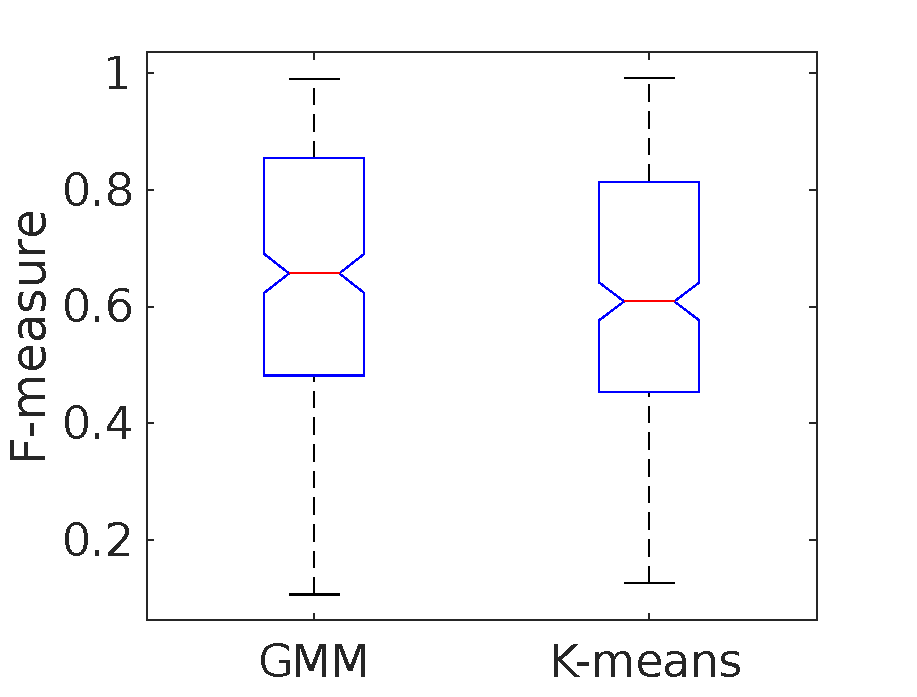
\includegraphics[height=3cm]{Figures/boxplot_method}
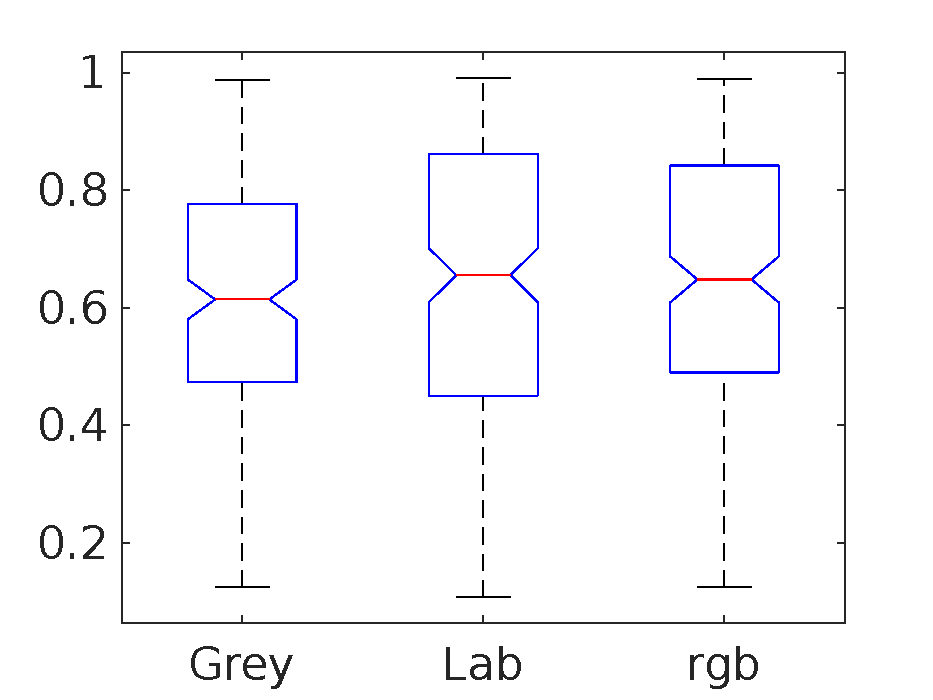
\includegraphics[height=3cm]{Figures/boxplot_space}
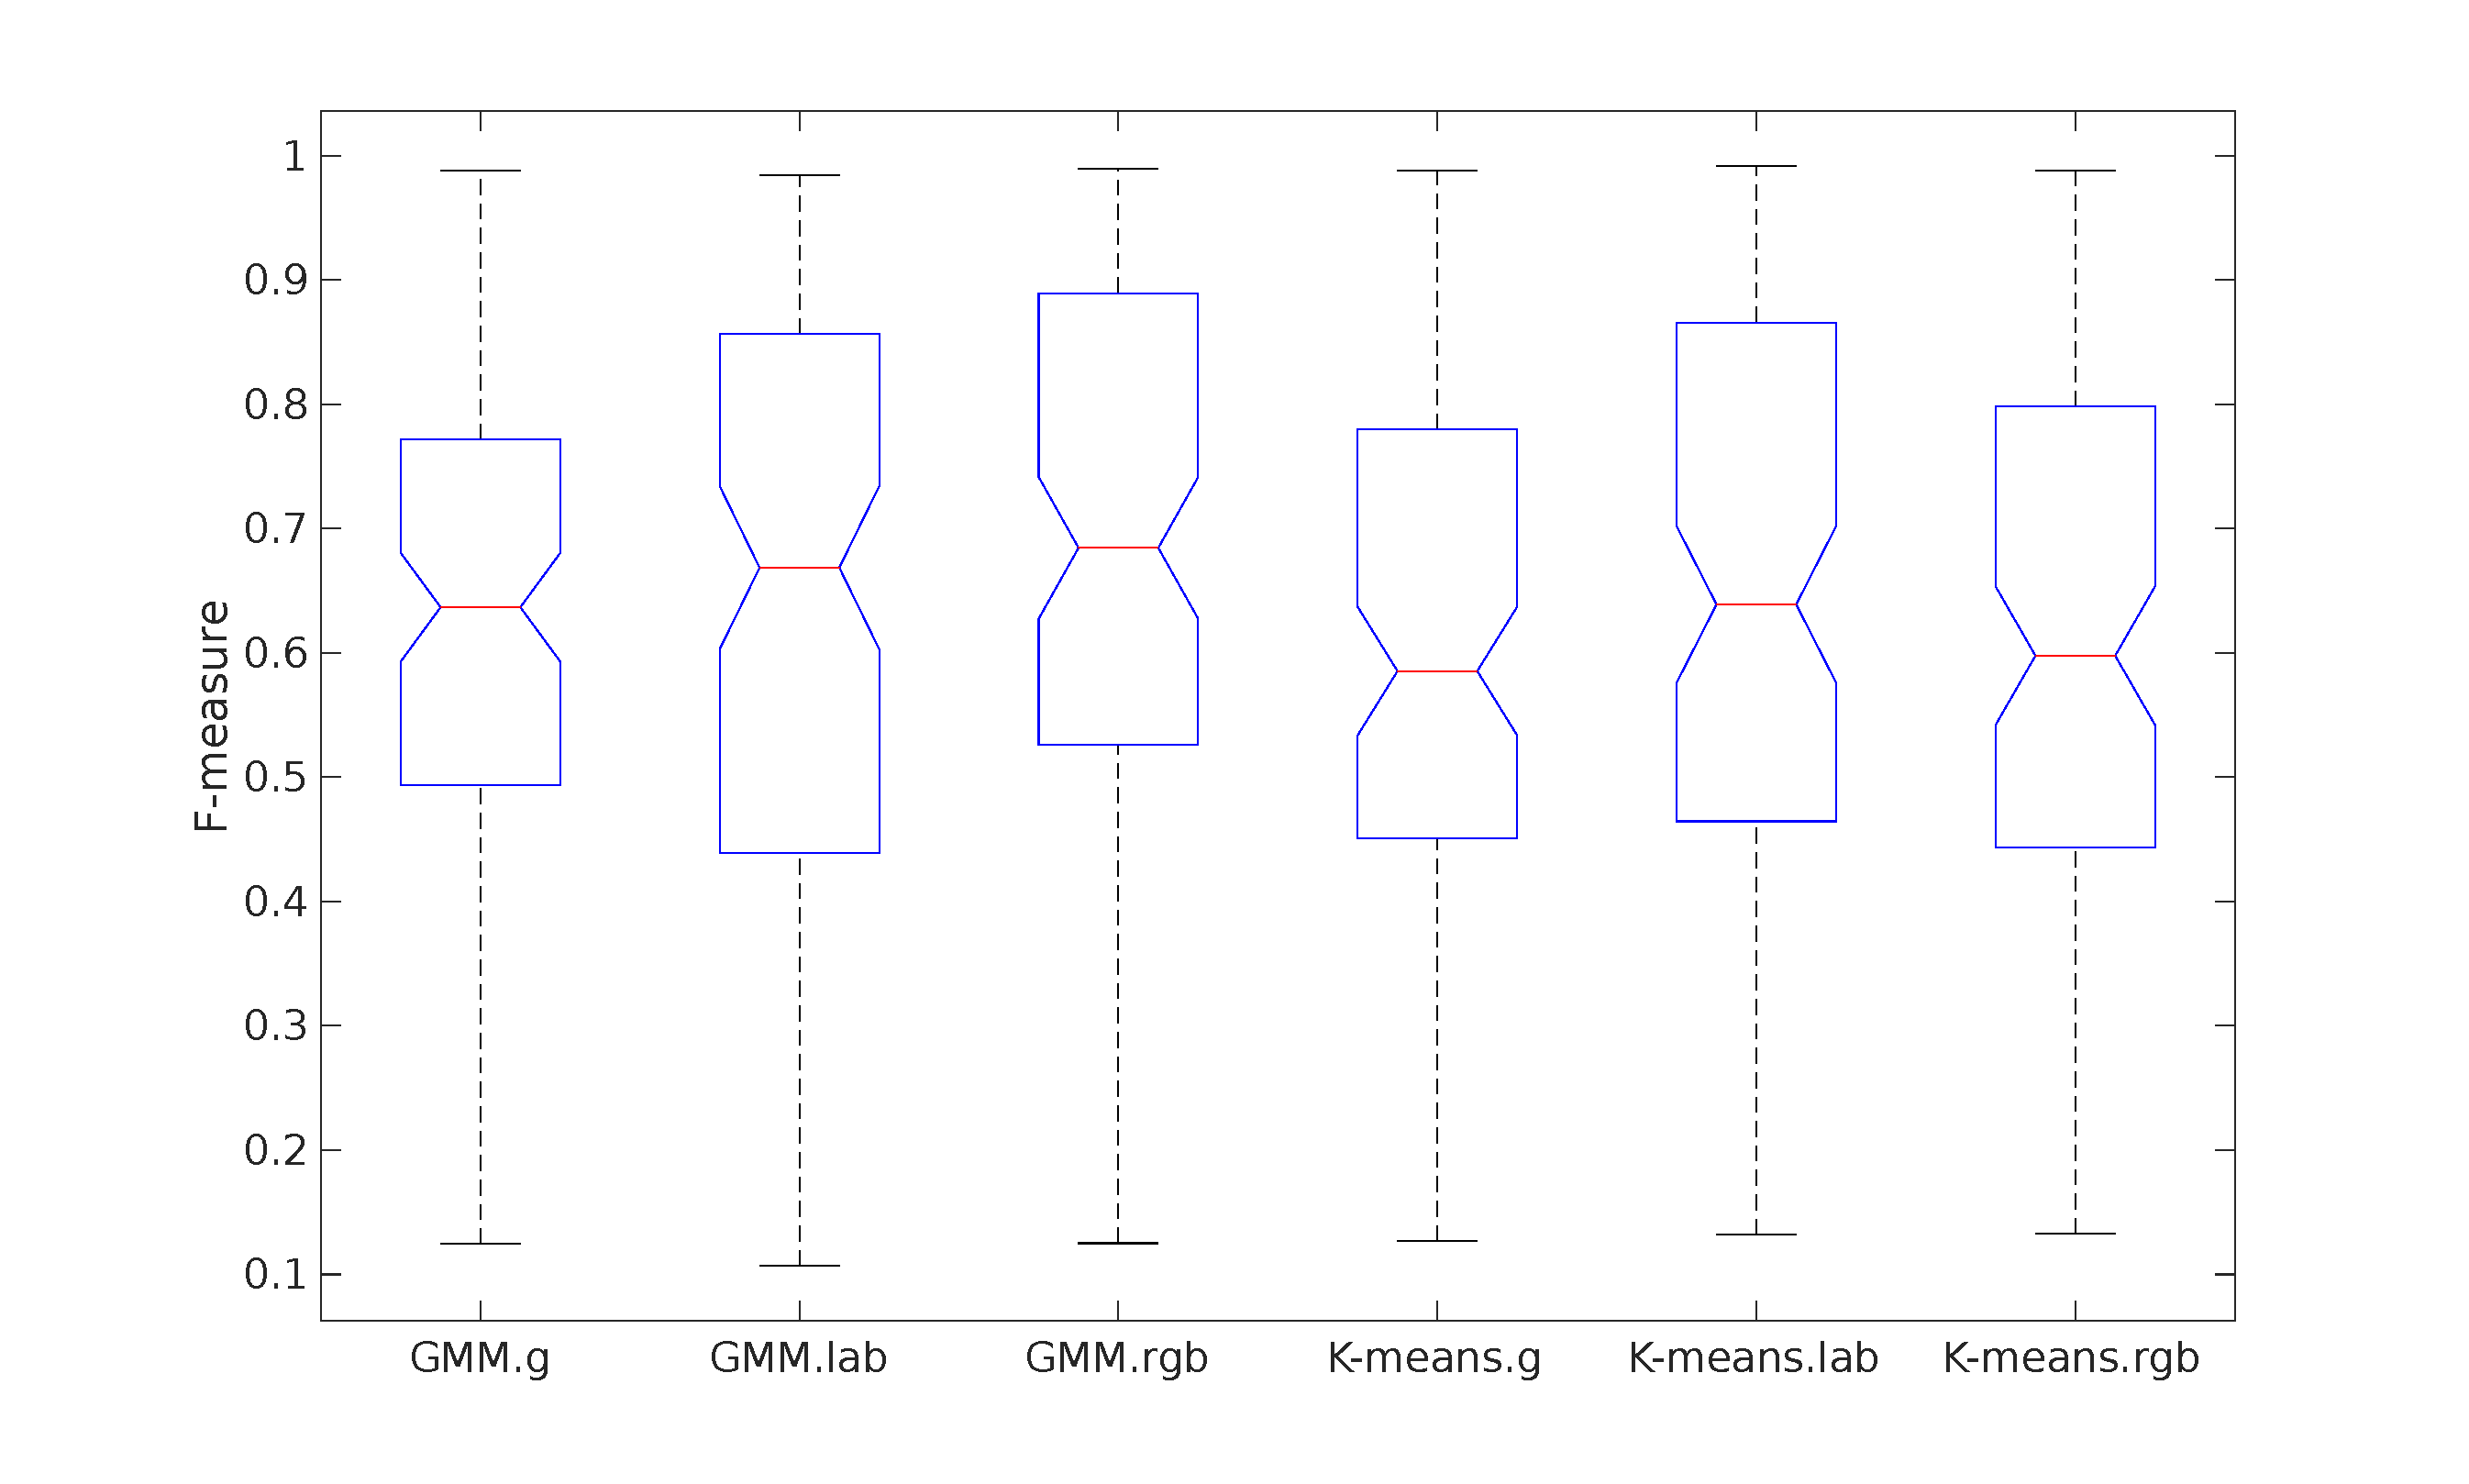
\includegraphics[height=3cm]{Figures/Fmeas_boxplot}
\caption{Box plots of differents groups and methods.}
\end{figure}

When looking more precisely to the all pairs, it can be seen that the GMM with rgb space significantly performs the best where the K-means with grey have the lowest F-score.  All the results allowed us to prove our first assumption  which was that the GMM rgb is better than the others.

\begin{table}
\centering
\caption{GMM.rgb versus all}
\label{tab:mtrebetween}
\begin{tabular}{l|ccccc}
\toprule
	&	GMM.g	&	GMM.lab	&	K-means.g 	&	K-means.lab	&	K-means.rgb\\
\cmidrule(lr){2-6}
$p$					&	$0.023$	&	$0.097$			&	$<0.001$	&	$0.017$	&	$0.037$\\
\bottomrule
\end{tabular}
\end{table}

To conclude, it is interesting to have some qualitative results when my GMM.rgb failed and when it worked. 
Some pictures are difficult to segment because the background and the object have the same color, and the GMM with two component is to poor to detect properly the object. For example the image `dscf0034\_l' of the charette is complicated, indeed the charette has the same color as the wheat field. The K-means perfoms better is this case because it is not smooth like the gmm and can detect object inside structures more easily.
\begin{figure}
\centering
\fbox{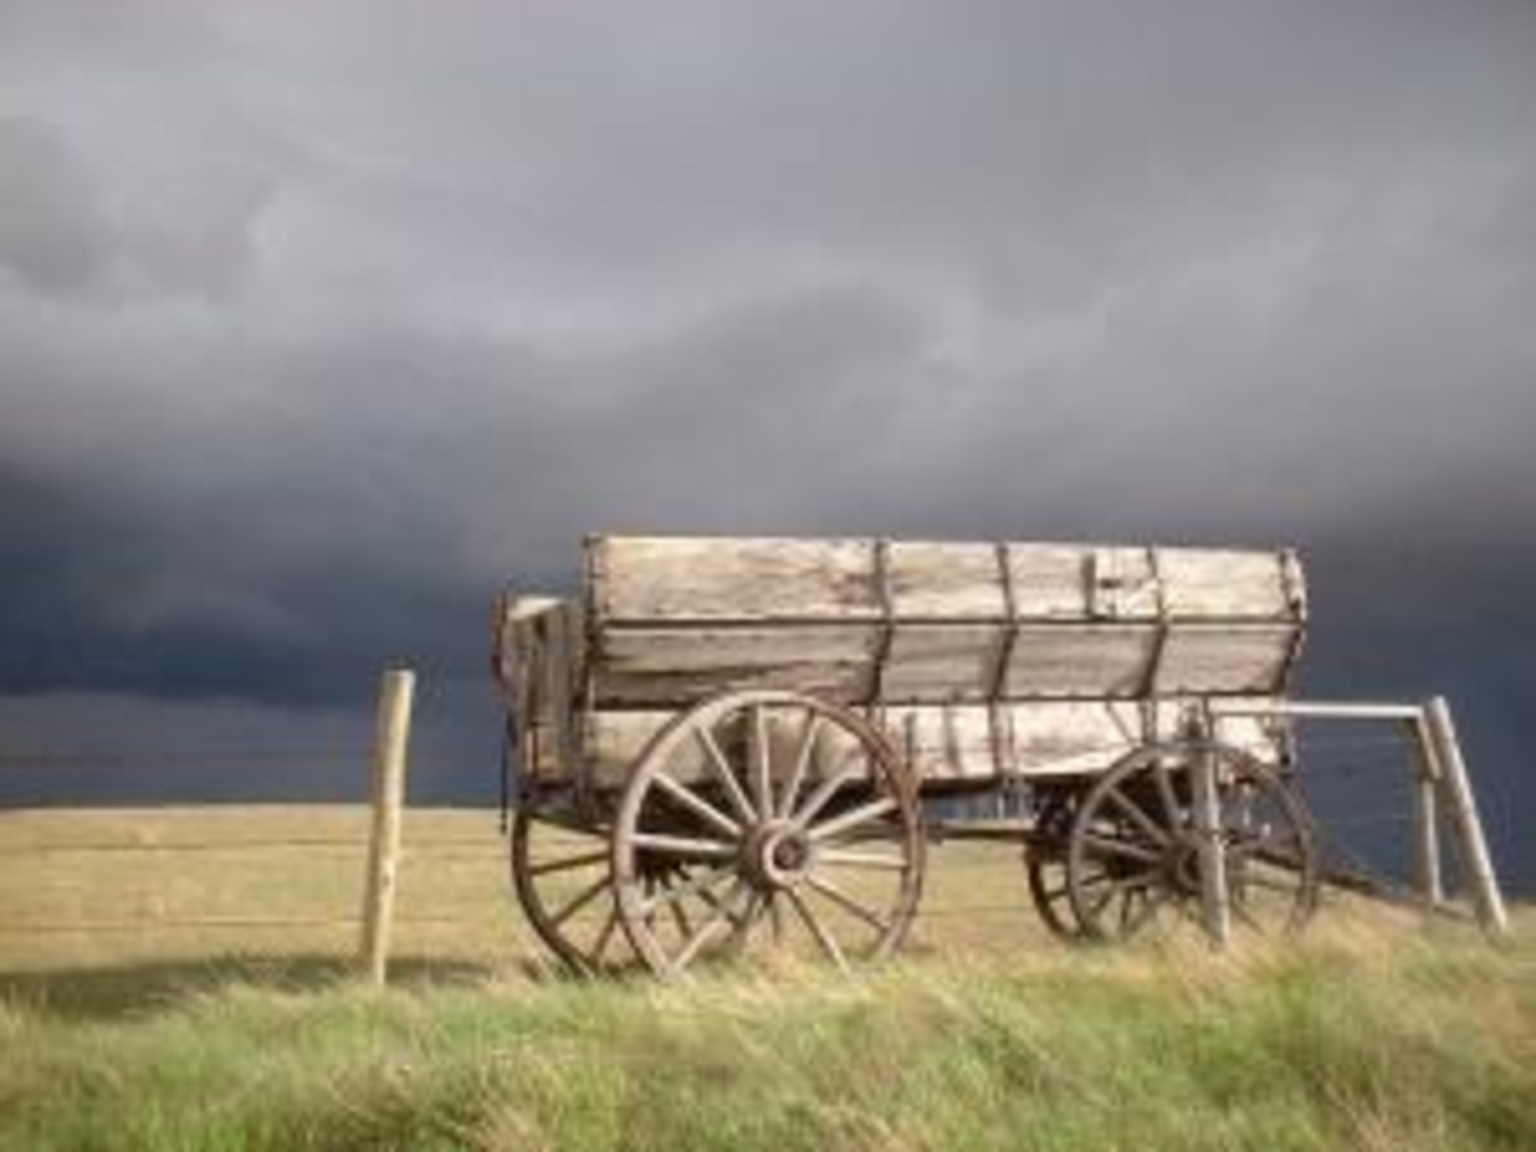
\includegraphics[height=2cm]{Figures/gmm_fail_image}}\qquad
\fbox{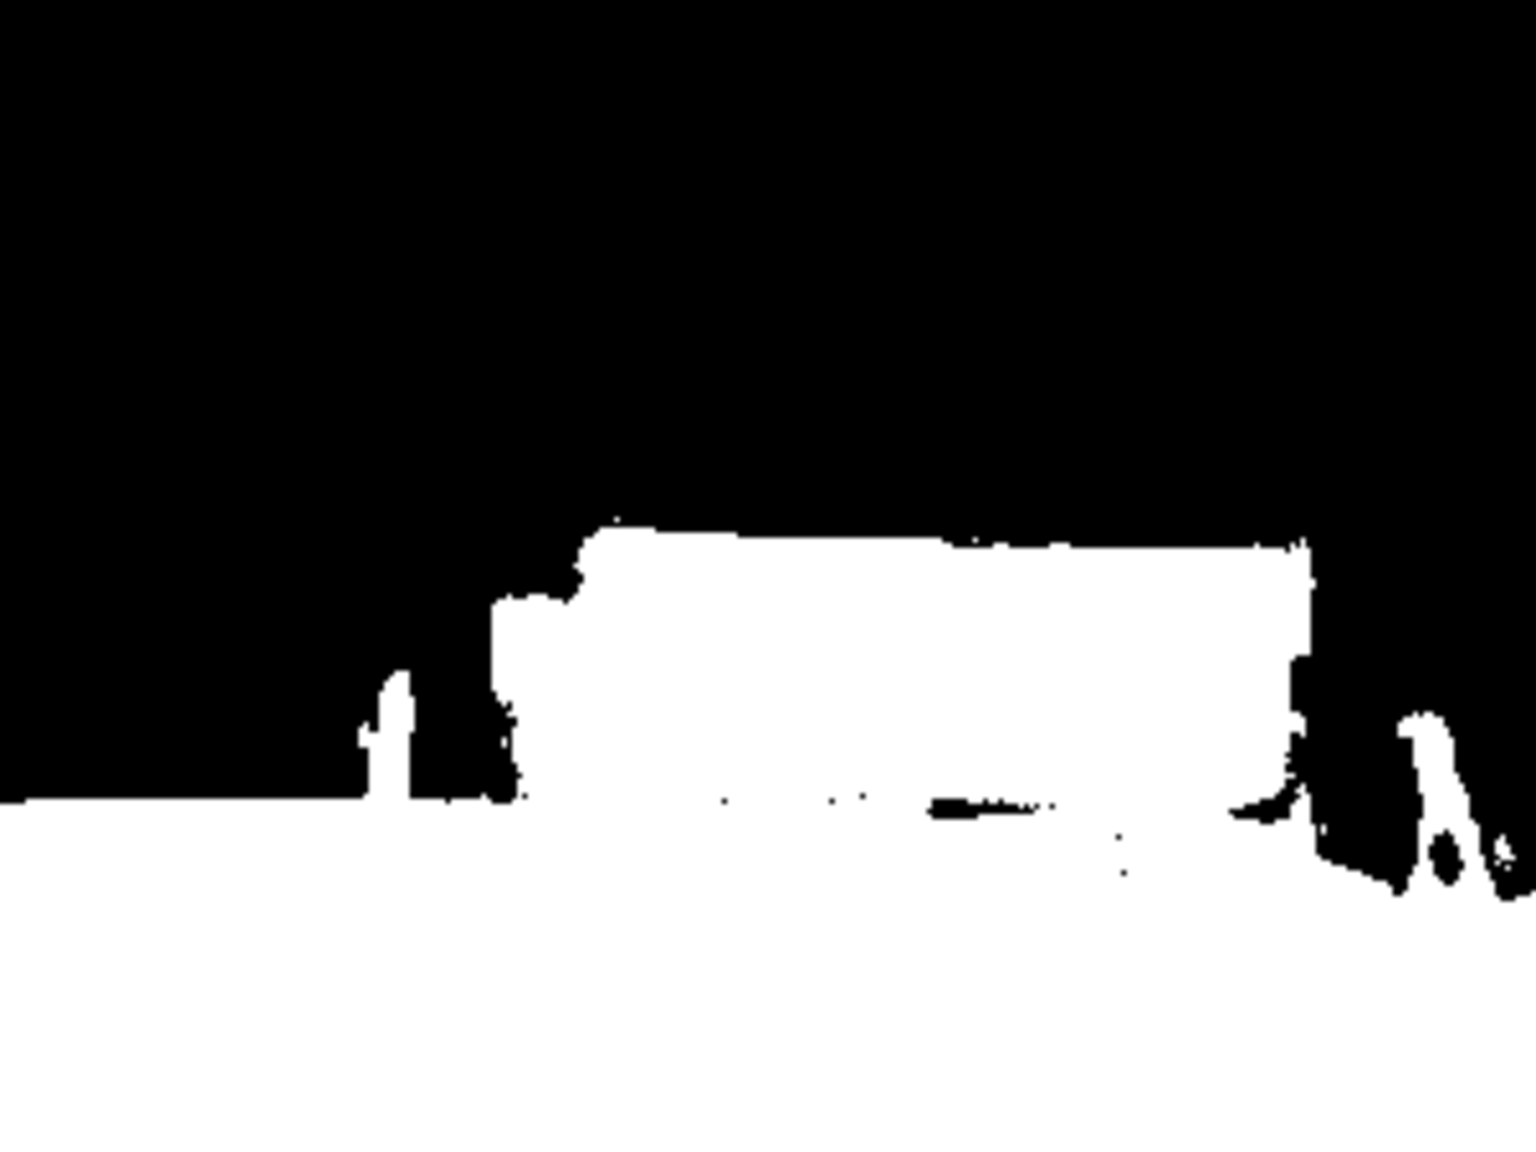
\includegraphics[height=2cm]{Figures/gmm_fail_res}}\qquad
\fbox{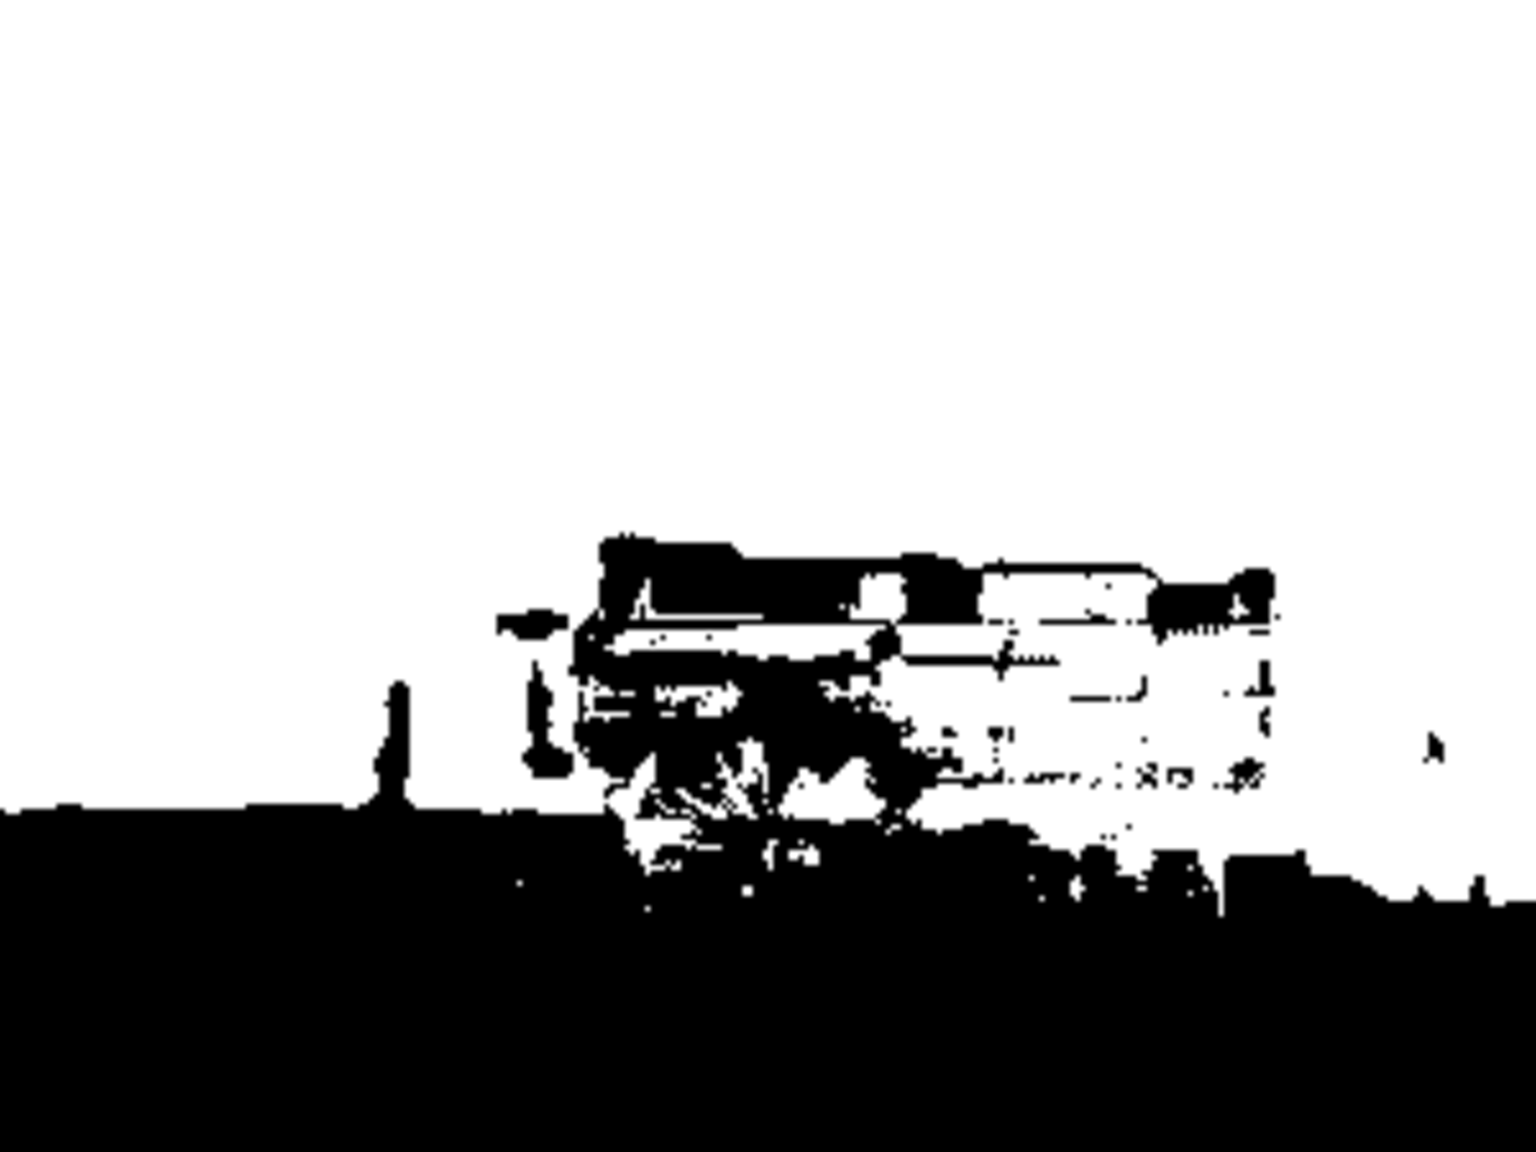
\includegraphics[height=2cm]{Figures/gmm_fail_res_k}}
\caption{Segmentation results of `dscf0034\_l' for GMM (middle) and K-means (right)}
\end{figure}

The picture `sharp\_image' is interesting for the GMM because its smoothness allowed to not detect the cactus peak, contrary to the K-means where it didn't perform well for this task. Moreover, some problems of covariance conditioning where detected for images with a wide black or white scene (like images `culzeancastle' or `pic1092515922117'). In these cases the K-means is better, because GMM's covariance matrix tend to refine to much. 
\begin{figure}
\centering
\fbox{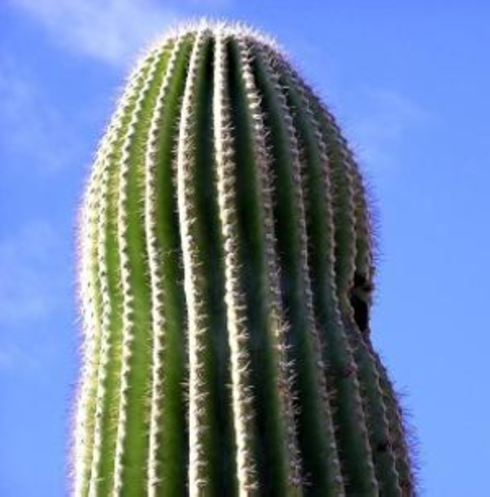
\includegraphics[height=2cm]{Figures/gmm_work_image}}\qquad
\fbox{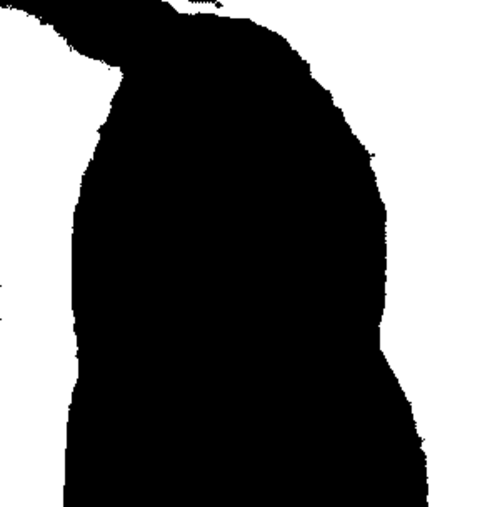
\includegraphics[height=2cm]{Figures/gmm_work_res}}\qquad
\fbox{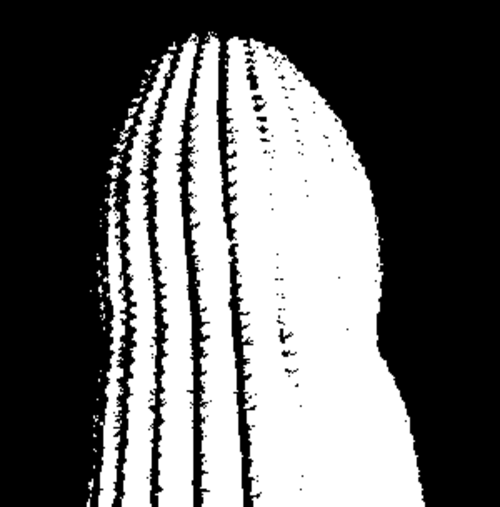
\includegraphics[height=2cm]{Figures/gmm_work_res_k}}
\caption{Segmentation results of `sharp\_image' for GMM (middle) and K-means (right)}
\end{figure}
\par Finaly, even if K-means has the poorest results, it can be really interesting for his fast computation time, cases where the background is intense and for low resolution images. In the other hand, the GMM is good when the image is more noisy (resolution is high) and perform well to extract little object. Knowing the drawbacks, it can be interesting to first use a K-mean to extract the object of the background in a high level of pyramid, and after use a GMM in the lowest floor of the pyramid to detect more easily the area of interest.

{\small
\bibliographystyle{splncs03}
\bibliography{assignment1}
}

\end{document}
